Model wspólnej pamięci składa się z pewnej liczby procesorów, z których każdy posiada własną pamięć i może lokalnie wykonywać programy. Wszystkie procesory mogą komunikować się za pomocą wspólnej globalnej pamięci (rys. \ref{fig:model_shared}).


Każdemu procesorowi przypożądkowana jest niepowtarzająca się liczba naturalna. Jest to lokalnie dostępny indeks, numer procesora lub jego identyfikator.

\begin{figure}[h]
\centering
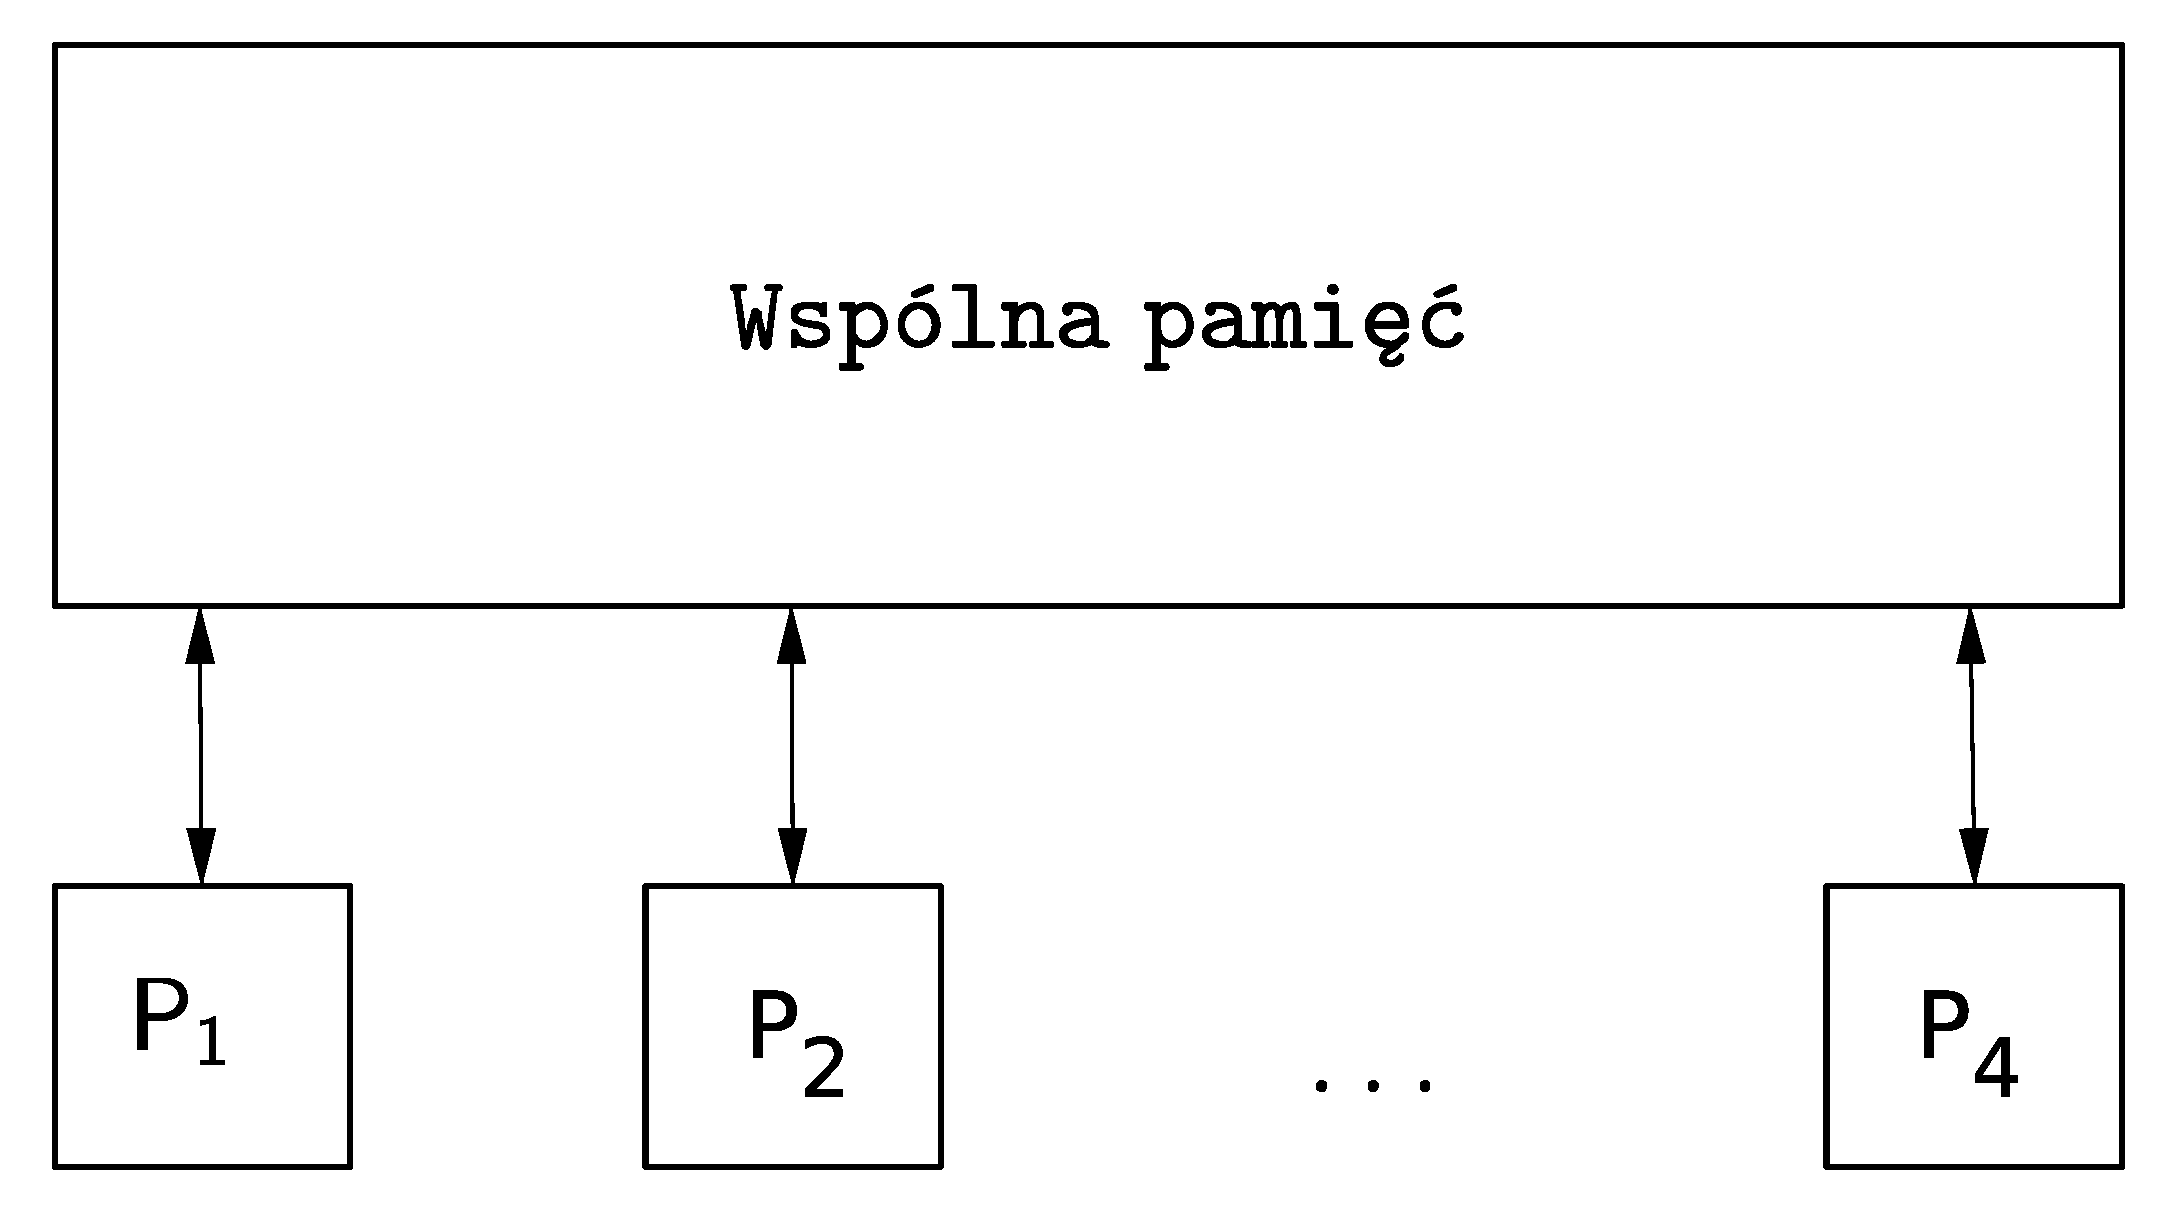
\includegraphics[width=20em]{images/Rys4.eps}
\caption{Model wspólnej pamięci}
\label{fig:model_shared}
\end{figure}

W modelu wspólnej pamięci wyróżniamy dwa podstawowe tryby operacji.
\paragraph{Tryb synchroniczny.} Wszystkie procesory działają synchronicznie według wspólnego zegara. Model ten nazywamy równoległą maszyną o dostepie swobodnym (PRAM, parallel random-access machine).


\paragraph{Tryb asynchroniczny.} Każdy procesor pracuje według osobnego zegara. W tym trybie programista jest odpowiedzialny za odpowiednią synchronizację procesorów, jeśli zachodzi taka potrzeba. Dokładniej mówiąc, jeśli procesor ma pobrać dane, to odpowiedzialnością programisty jest upewnienie się, że odpowiednie dane są już uzyskane, ponieważ wartości wspólnych zmiennych są określane dynamicznie w trakcie wykonania programu na różnych procesorach.


Ponieważ każdy procesor może uruchomić swój program lokalnie, ten model jest typu MIMD w klasyfikacji Flynna. Znaczy to tyle, że każdy procesor może wykonać pewną instrukcję lub operację na danych niezależnie od tych wykonanych na jakimkolwiek innym procesorze w trakcie danej jednostki czasu.


Dla danego algorytmu, rozmiar danych wymienionych pomiędzy pamięcią globalną i pamięcią lokalną różnych procesorów wyraża rozmiar \textbf{komunikacji} wymaganej przez algorytm.


Możemy wyróżnić kilka wariantów modelu PRAM w zależności od wymagań jakie postawimy odnośnie jednoczesnego dostępu kilku procesorów do tego samego adresu w pamięci globalnej.\\
\begin{itemize}
\item\textbf{EREW} -- algorytmy z wyłącznym odczytem i wyłącznym zapisem; nie pozwala na jednoczesny zapis do pamieci.
\item\textbf{CREW} -- algorytmy z jednoczesnym odczytem i wyłącznym zapisem; pozwala na jednoczesny  dostęp do pamięci dla instrukcji odczytu.
\item\textbf{CRCW} -- algorytmy z jednoczesnym odczytem i jednoczesnym zapisem.
\item\textbf{ERCW} -- algorytmy z wyłącznym odczytem i jednoczesnym zapisem.
\end{itemize}


Jeśli nie poczyni się żadnych dodatkowych założeń, to nie jest jasno określone, co zostanie zapisane w komórce pamięci w wyniku jednoczesnego zapisywania do niej przez wiele procesorów w algorytmie typu CRCW. W literaturze można spotkać wiele typów maszyny PRAM, które różnią się sposobami rozwiązywania konfliktów zapisu. Można wśród nich wyróżnić\cite{Cormen94}:
\begin{enumerate}
\item jednolity (ang. common) – procesory muszą zapisać do tej samej komórki pamięci jednolitą wartość
\item dowolny (ang. arbitrary) – zapamiętywana jest dowolna wartość z wartości zapisywanych do tej samej komórki pamięci
\item priorytetowy (ang. priority) – zapamiętywana jest wartość zapisywana przez procesor o najmniejszym numerze
\item (ang. combining) – zapamiętywana jest wartość jest pewną, jednak ściśle określoną kombinacją zapisywanych wartości
\end{enumerate}

